\documentclass{article}
\usepackage{tikz} % for creating flowcharts
\usetikzlibrary{shapes}
\usetikzlibrary{arrows.meta}
\usetikzlibrary{arrows}

\usepackage{enumitem} % for customizing lists
\usepackage{hyperref} % for adding hyperlinks
\usepackage{tcolorbox}
\usepackage[a4paper]{geometry} % set the page size to A4
\geometry{left=2.5cm,right=5cm,top=2.5cm,bottom=2.5cm} % set the margins to 2.5cm
\usepackage{marginnote} % for adding margin notes

\begin{document}

\title{Operational Procedures and Processes}
\author{Your Name Here}
\date{\today}

\maketitle

\tableofcontents

\section{Introduction}
Introduce the purpose of the document and give an overview of the operational procedures and processes that will be discussed.

\section{Procedures}

\subsection{Procedure 1}

\begin{tcolorbox}[colback=yellow!10!white,colframe=yellow!70!black,title=Important Note]
    This is some important information that should be highlighted in a box.
\end{tcolorbox}

Describe the first procedure here.
% add a margin note
\marginnote{
    This is a note in the margin. You can write anything you want here.
}
\begin{enumerate}[label=\alph*.]
    \item Step 1
    \item Step 2
    \item Step 3
\end{enumerate}

\newpage    

\marginnote{
    This is a note in the margin. You can write anything you want here.
}
% create the flowchart using tikz
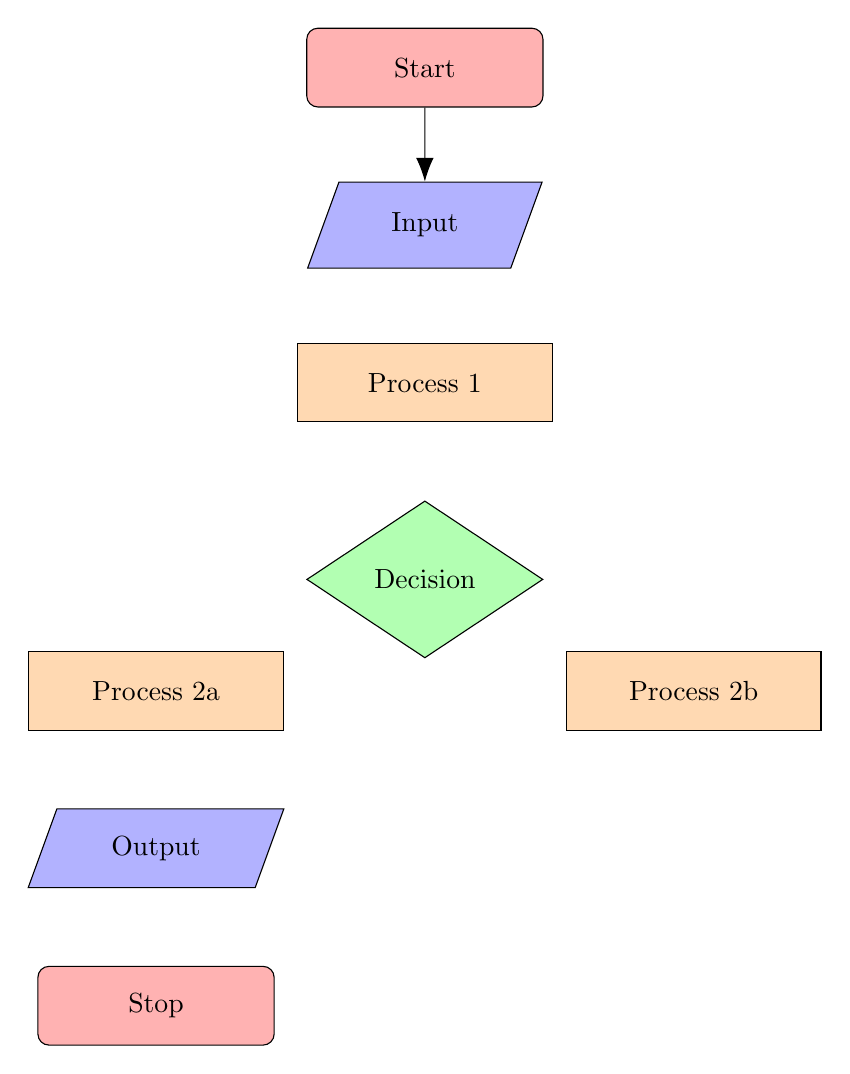
\begin{tikzpicture}[node distance=2cm]
\tikzstyle{line}=[draw] % here

\tikzstyle{startstop} = [rectangle, rounded corners, minimum width=3cm, minimum height=1cm, text centered, draw=black, fill=red!30]
% Define the io style for input/output nodes
\tikzstyle{io}=[trapezium,trapezium left angle=70,trapezium right angle=-70,minimum width=3cm,minimum height=1cm,text centered,draw=black,fill=blue!30]

% Define the process style for process nodes
\tikzstyle{process}=[rectangle,minimum width=3cm,minimum height=1cm,text centered,text width=3cm,draw=black,fill=orange!30]

% Define the decision style for decision nodes
\tikzstyle{decision}=[diamond,minimum width=3cm,minimum height=1cm,text centered,draw=black,fill=green!30]

% define the nodes in the flowchart
\node(start)[startstop]{Start};
\node (input) [io, below of=start] {Input};
\node (process1) [process, below of=input] {Process 1};
\node (decision) [decision, below of=process1, yshift=-0.5cm] {Decision};
\node (process2a) [process, below left of=decision, xshift=-2cm] {Process 2a};
\node (process2b) [process, below right of=decision, xshift=2cm] {Process 2b};
\node (output) [io, below of=process2a] {Output};
\node (stop) [startstop, below of=output] {Stop};

% define the arrows between the nodes
\draw[-{Latex[length=3mm]}] (start) -- (input);

% \draw[arrow] (start) -- (input);
% \draw[arrow] (input) -- (process1);
% \draw[arrow] (process1) -- (decision);
% \draw[arrow] (decision) -- node[anchor=east] {Yes} (process2a);
% \draw[arrow] (decision) -- node[anchor=west] {No} (process2b);
% \draw[arrow] (process2a) -- (output);
% \draw[arrow] (output) -- (stop);
% \draw[arrow] (process2b) |- (stop);

\end{tikzpicture}


\subsection{Procedure 2}
Describe the second procedure here.

\begin{enumerate}[label=\alph*.]
    \item Step 1
    \item Step 2
    \item Step 3
\end{enumerate}

\section{Processes}

\subsection{Process 1}
Describe the first process here.

\begin{itemize}
    \item Step 1
    \item Step 2
    \item Step 3
\end{itemize}

\subsection{Process 2}
Describe the second process here.

\begin{itemize}
    \item Step 1
    \item Step 2
    \item Step 3
\end{itemize}

\section{Conclusion}
Summarize the operational procedures and processes described in the document.

\end{document}
